

%\begin{sidewaysfigure}
%\centering
%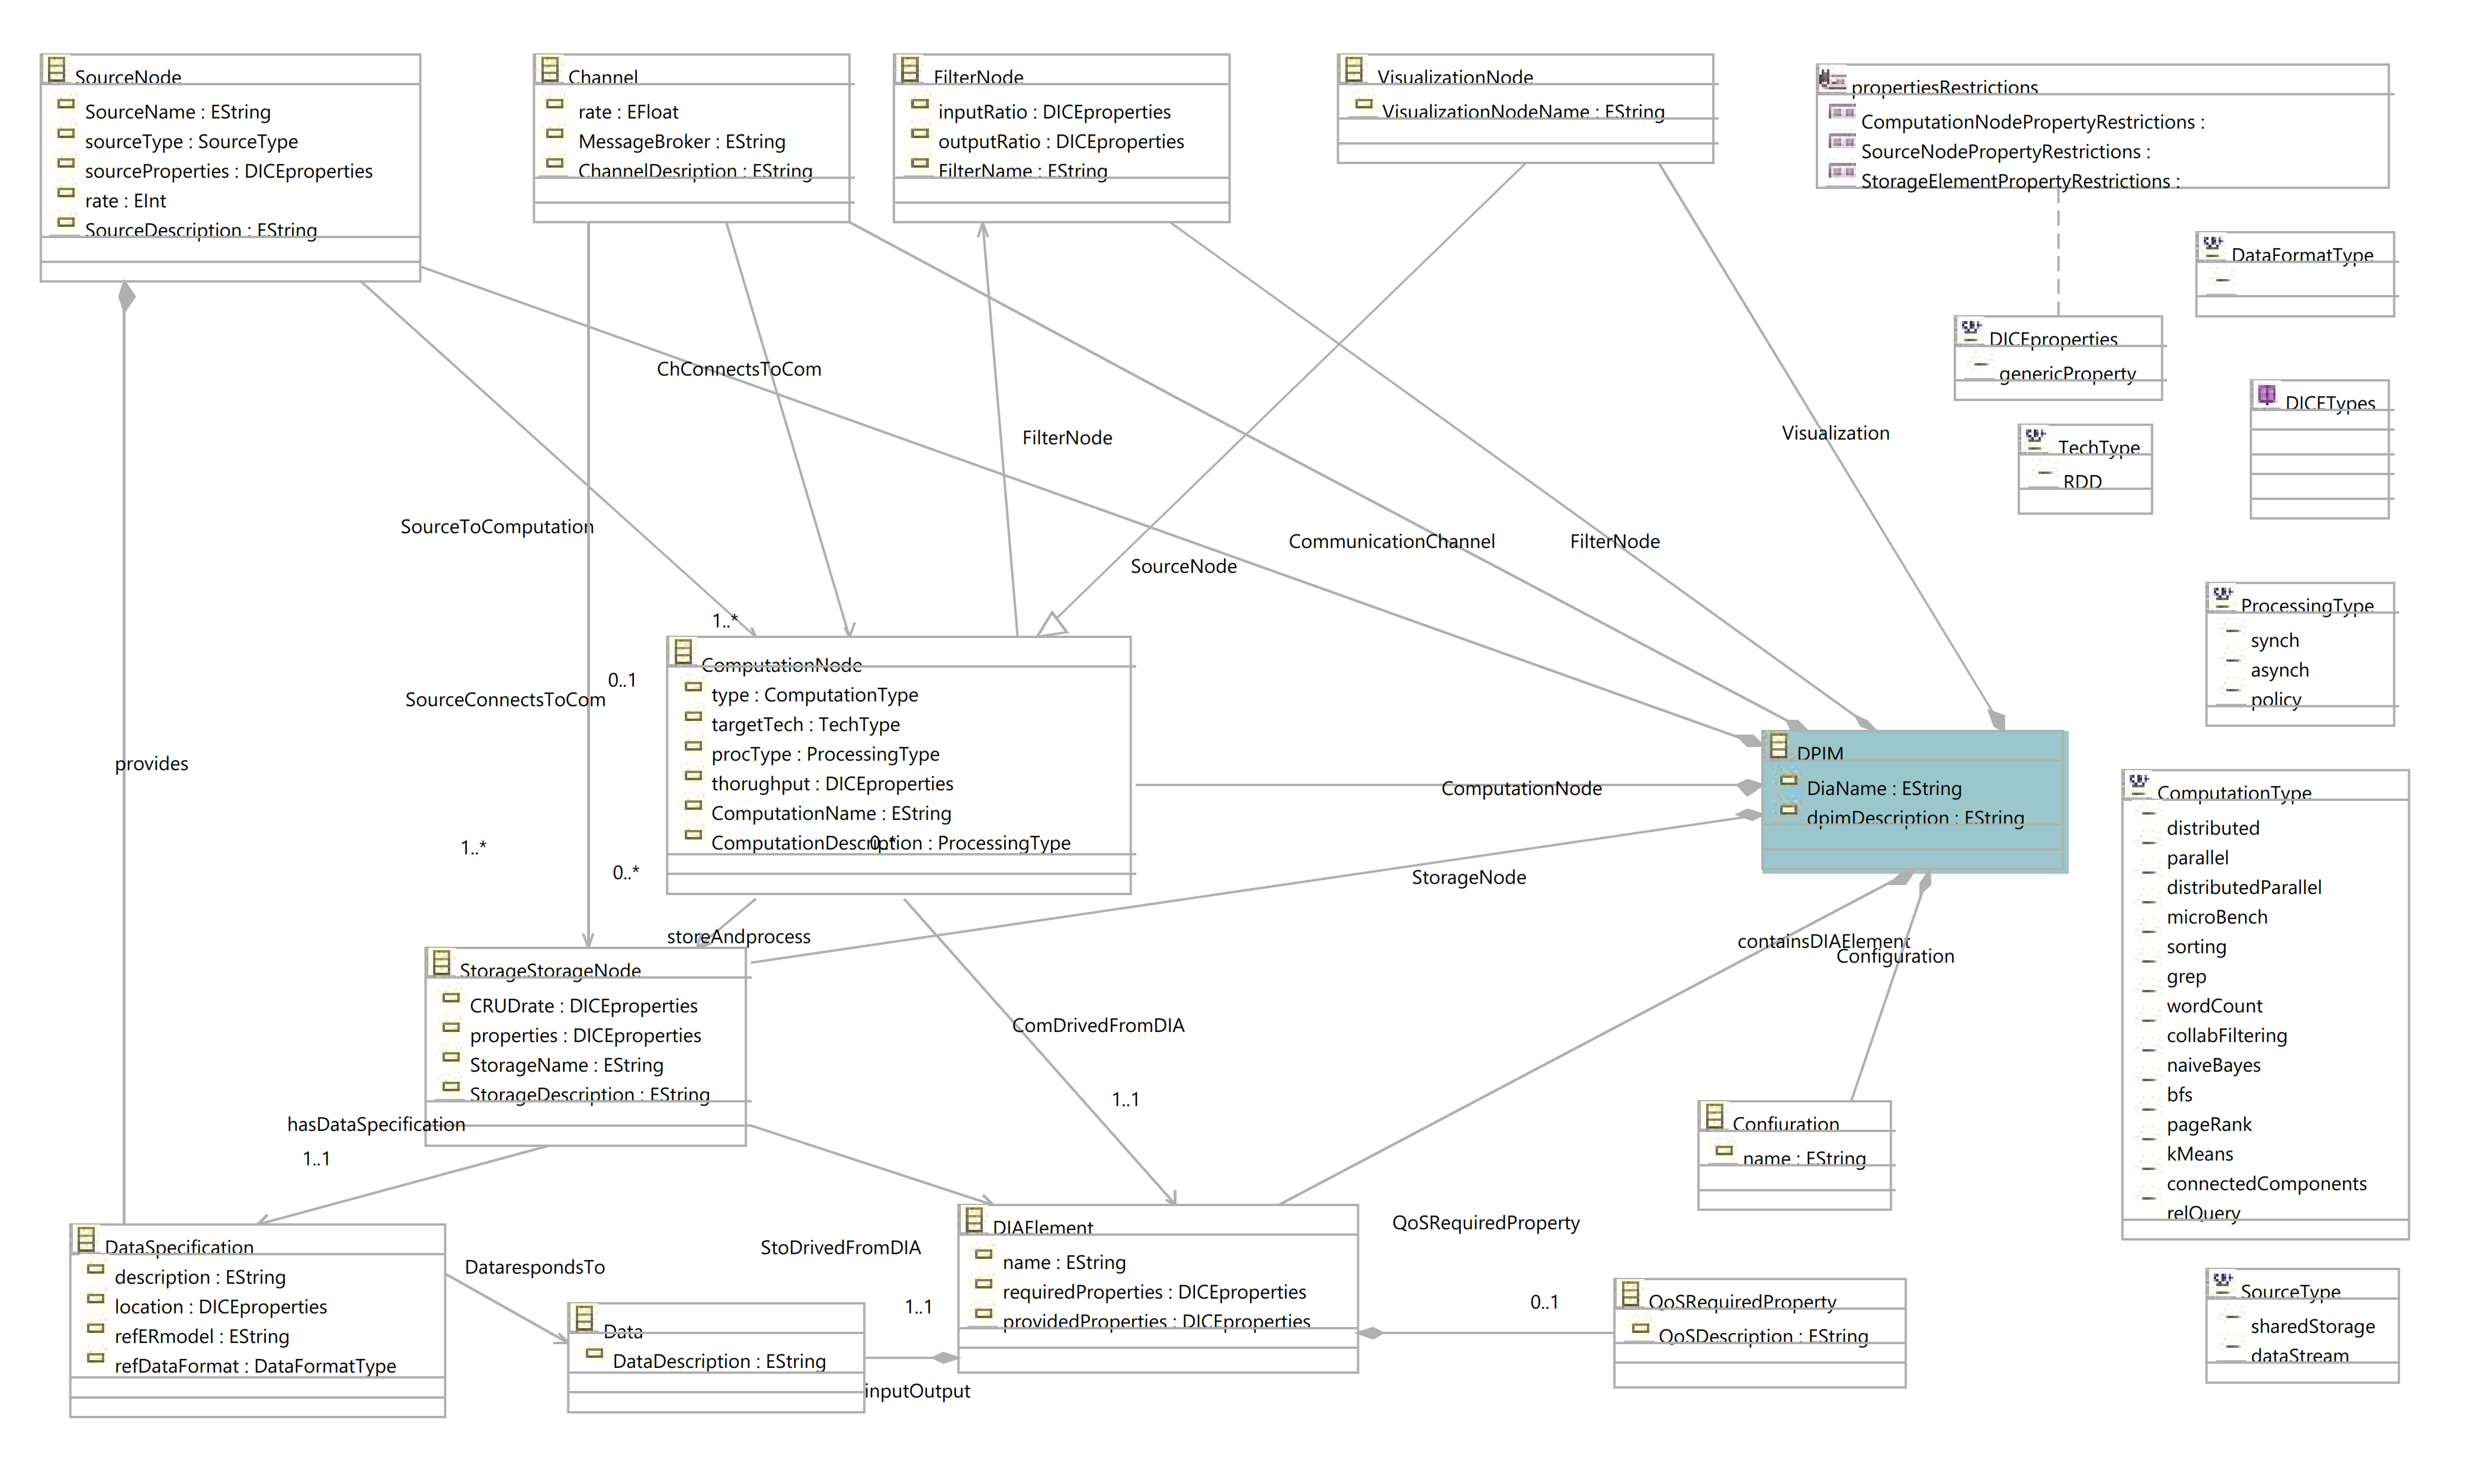
\includegraphics[width=\textwidth]{Images/11.png}
%\caption{\label{fig:metamodel}DICE DPIM metamodel.}
%\end{sidewaysfigure}

%\begin{figure}
%\centering
%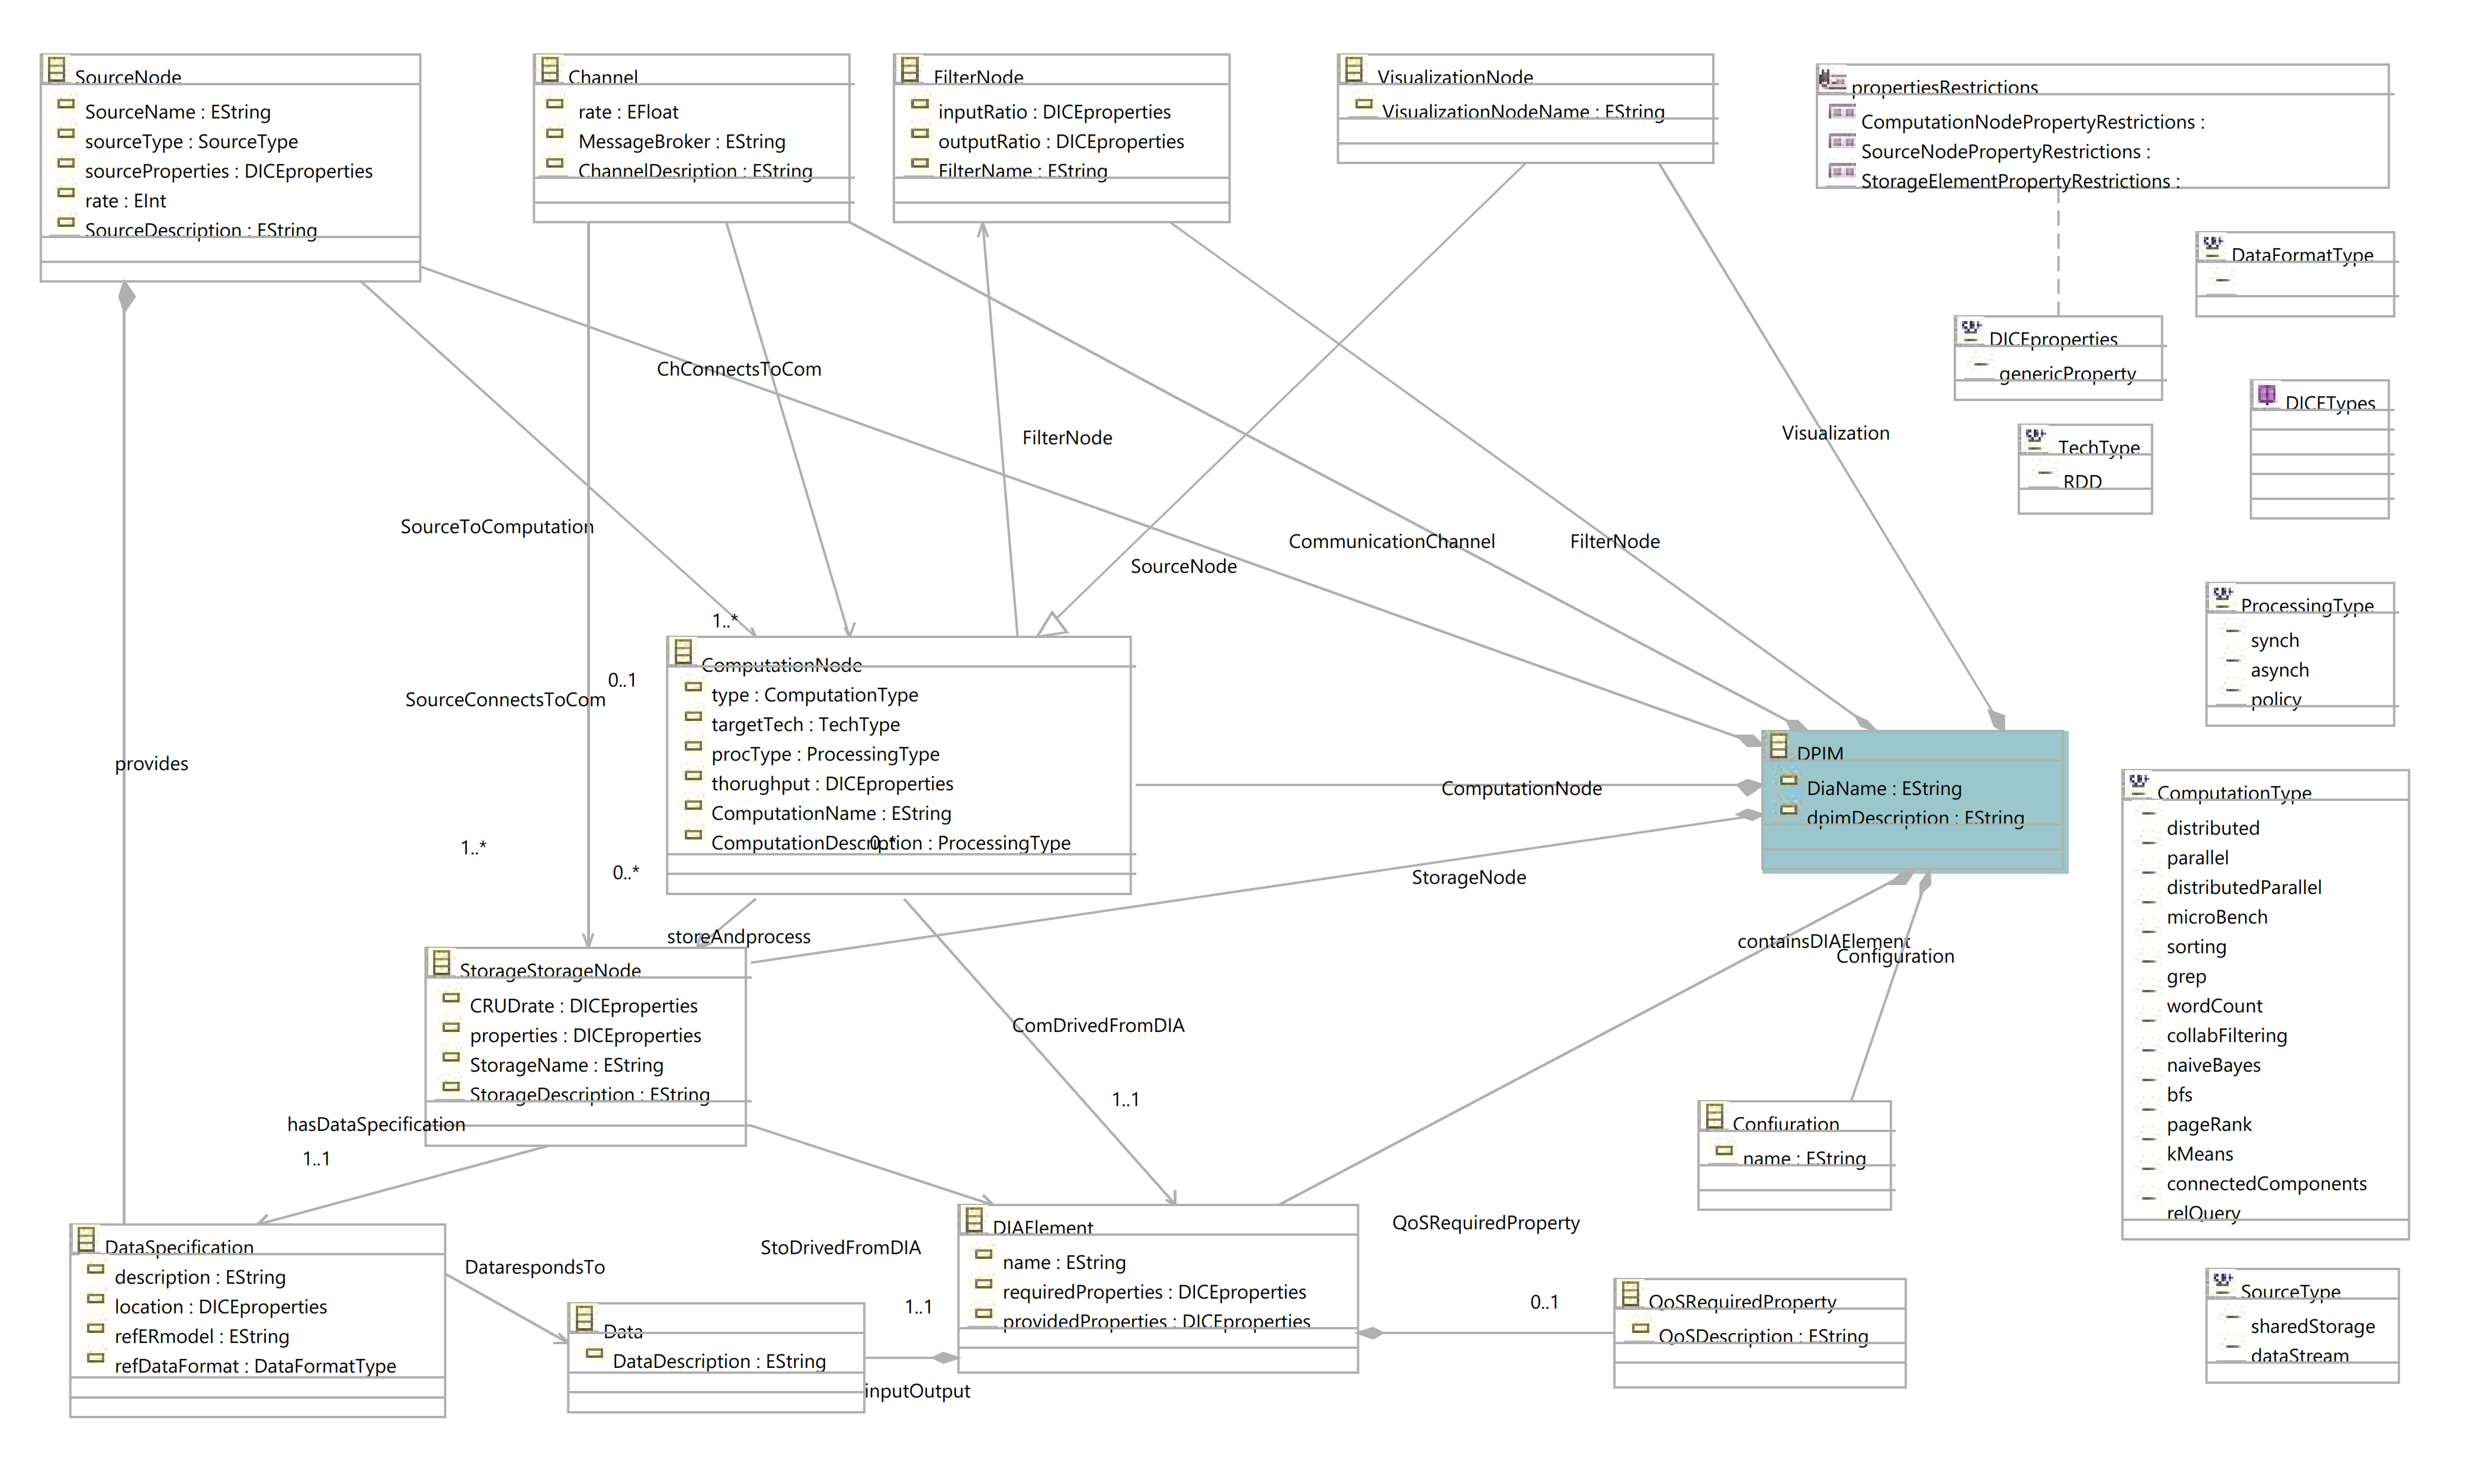
\includegraphics[width=\textwidth]{Images/11.png}
%\caption{\label{fig:metamodel2}DICE DPIM metamodel in portrait form.}
%\end{figure}

\subsection{Product perspective }


add here class diagram + verbal description



%add a state diagram for each subsect


\subsection{Product functions}

\subsubsection{login }
\subsubsection{sending pics}
\subsubsection{Explore Data}
The app will offer the possibility to the users to visualize the data collected.
Two kind of visualizations are offered:
\begin{enumerate}
  \item Streets with the highest frequency of violations
  \item Veichles that committed the most violations
\end{enumerate}
In order to get those data the system will periodically query the database of violations in order to create a table where the count of violation is stored, both for streets and veichles.
There will be a section in the app called "Explore Data" where will be able to choose which kind of data to visualize.



\subsubsection{Issue a ticket }
Every time a new violation is inserted in the database, the System will use the new data available to generate a proposal of ticket, combining the data from violations with data coming from Municipality databases.

A ticket has the following structure:
\begin{enumerate}
  \item Place where violation occurred
  \item Date when violation occurred
  \item Plate of veichle
  \item Article and code of violation
  \item Amount to be paid
  \item Date when the payment is due
\end{enumerate}

The ticket will be in a pending-approval status because we want always an human check before sending it to the offender.
Authority users (e.g. policemans) will check the pending-approval tickets and they can approve them or not.
If ticket is not approved it will go in approval-denied status
If ticket has been approved it will have to be sent to the offender.
The system will connect to the external vehicle registration database in order to retreive the name, surname, address of the offender knowing the licence plate of his/her veichle.
Now we have all the data to print the ticket and send it via regular mail. There will be an office of policestation which will do the job.

\subsubsection{generate statistics}

\subsection{User characteristics }


\subsection{Assumptions, dependencies and constraints}
\begin{enumerate}
\dom{}  Device has internet connection
\dom{1} The device should acquire position with an accuracy of enouth meters in order to univocally determine the road (e.g. 5 meters)
\dom{} We have access to an ALPR service which is able to read every licence plate in a picture and return the string
\dom{1} The device should take pictures with enouth resolution to be able to read by the ALPR service
\dom{5} ALPR service has an accuracy of more than 90\%
\dom{2} Every veichle that can be reported shoud have a licence plate visible
\dom{3} The number and kind of violations should be finite (defined by the law)
\dom{4} Every authority account is verified and it's not possible to be created using the frontend
\dom{6} We have access to the vehicle registration database where are stored licence plates, names and the addresses of the owners of every veichle registered
\dom{7} We have access to a database where are stored all the codes of violations and the amount of fine for the violation

\end{enumerate}

The app will be dependent on a third-party service to read the licence plate of the cars. (For example \url{http://www.openalpr.com} )


The app will be dependent on a smartphone, which has to provide the following features:
\begin{enumerate}
  \item Internet connection, possibily using 2G/3G/4G in order to be available where there is no WiFi, considering the use case "on the road"
  \item GPS sensor
\end{enumerate}
